\documentclass{acmsiggraph}

\usepackage[scaled=.92]{helvet}
\usepackage{times}
\usepackage{graphicx}
\usepackage{parskip}
\usepackage{fixltx2e}
\usepackage[labelfont=bf,textfont=it]{caption}

\TOGonlineid{0}

\title{Obstacle Avoidance for a Quadrotor}

\author{Nikoli Dryden \thanks{dryden2@illinois.edu} %
\and Bryan Plummer \thanks{bplumme2@illinois.edu}}
\pdfauthor{Nikoli Dryden}

\begin{document}

\maketitle

\begin{abstract}
We implement and evaluate the approach of~\cite{lee2011} for obstacle avoidance for an ARDrone 2 quadrotor, which integrates MOPS and SIFT features to get a sparse representation of obstacles. We also evaluate the existing PTAM~\cite{klein07parallel} approach to UAV navigation. We find that the MOPS features are not robust on the quadrotor's data and that the Lee at al. approach is both ineffective and computationally intensive whereas the PTAM system achieves robust, real-time performance.
\end{abstract}

\section{Introduction}
Micro aerial vehicles(MAV's), which include quadrotor and unmanned aerial vehicles(UAV's), have the potential to become more 
prominent over the next several years.  These aircraft allow easy access for many places which are difficult for humans 
to go in a safer manner for both humans and the environment and have applications reaching into search and rescue, tracking,
mapping, and others.  In order for the higher level tasks to be handled these vehicles must have a reliable 
navigation system.

There are GPS solutions for navigation work out of the box (e.g. the AscTec series of quadrotors), but are limited in use
to locations where GPS is available.  While much progress has been made to solve to create a navigation solution
for these cases, we still strive to have a system that works in unknown, GPS denied, and cluttered environments.  As many 
MAV's are limited in both carrying capacity and power, laser range finders are too heavy and consume too much power to be of 
use. Stereo camera's become highly inaccurate after a set distance rendering them of no more use than using a single camera.

The common structure from motion approach to visual navigation using a single camera has been shown to suffer from some 
drawbacks.  In order to generate a 3D map, two types of camera translation may be necessary~\cite{shah2010}.  While
a quadrotor may be capable of such a maneuver, a UAV is not.  In~\cite{shah2009} the amount of computation required using this 
approach increased by about 15 times with only an increase from 8 to 35 feature points, and the number of features in a real
scene can number in the hundreds or thousands.

As an attempt to solve this problem~\cite{lee2011} proposed an approach to reduce the number of points required to 
represent the 3D structure of a scene.  The authors used multiscale oriented patches(MOPS)~\cite{BSW05} to create outlines of 
objects.  Since the outlines themselves are unable to tell if an outline is empty or not, they used the 3D location of SIFT 
features~\cite{lowe2004} located within the outlines to obtain this information.  

Although the proposed method cited collision avoidance for a quadrotor as its intended application, the authors did not 
dispense any data on its effectiveness in real scenes from images taken using a quadrotor.  This paper provides just such an 
evaluation using images taken from the AR-Drone 2.0 quadrotor with the processing being performed on a laptop obtaining the 
images from the quadrotor through a wireless network. In addition, we evaluate the use of the parallel tracking and 
mapping(PTAM)~\cite{klein07parallel} approach that was adapted as an online solution for quadrotors in~\cite{weiss2011}.

\section{Related Work}
Due to weight and energy restrictions aboard MAV's a vision based approach is seen as one of the most viable navigation 
solutions in GPS denied environments.  Progress in using visual senors for navigation purposes include performing specific 
tasks such as in~\cite{johnson2005} where a single camera was used to guide and land a MAV, or~\cite{huang2011isrr} where an 
RGB-D camera was used to map an environment and localize a quadrotor within that map but is restricted for use in indoor
environments.

Another common approach in the literature uses optical flow to estimate the relative motion between the frames of a camera.
In these systems one is able to detect collisions by measuring the relative rate of expansion of objects.  This method 
behaves poorly when light intensity doesn't remain constant~\cite{horn1981} and tends to be sensitive to noise and
an unstable camera.  As all MAV's will contribute to some vibrations in the camera this leads to inaccurate estimates in
flow vectors.

Some recent work attempts to use image segmentation to identify an obstacle and build a dense map around it~\cite{ha2012}.  
This approach shares some motivations as the first method attempted in this work in that it attempts to reduce the number
of computations required for navigation by using a limited number of feature points.  As with~\cite{lee2011}, this approach
has only been evaluated on theoretical data.  The authors note that in some cases image segmentation is not possible and 
intend to evaluate and extend their work to ascertain the extent this kind of information is beneficial to navigation.

\section{Approach}
We begin by describing our implementation of the approach in~\cite{lee2011}. Subsequently, we introduce a variation we attempted to generate an improved 3D map than we obtained using the unmodified version of~\cite{lee2011}.  Lastly, we describe our integration of the PTAM system with the quadrotor.

\subsection{Lee et al.'s Method}
Our approach closely follows that in~\cite{lee2011}. The goal is to make use of MOPS features to limit the number of SIFT features necessary for computing structural information about obstacles. We begin by assuming that we have, as input, two images taken from the quadrotor's forward-facing camera, that the images are of the same scene, and contain corresponding features. For our purposes, we need only a greyscale image and so discard the colour information.

In each image, we compute MOPS descriptors~\cite{BSW05}. The descriptors are located at features detected by a multi-scale Harris corner detector. Each descriptor is an $8 \times 8$ patch of bias/gain normalized intensity values and is oriented using a blurred local gradient. Feature density is controlled using an adaptive non-maximal suppression algorithm. SIFT descriptors~\cite{lowe2004} are also computed, using the OpenCV computer vision library *** CITE OpenCV ***.

Descriptors in these two images are then matched in order to generate putative matches. For MOPS, matching is performed using a brute-force matcher, since existing $k$-d tree implementations in OpenCV do not support efficient dynamic modification after creation. SIFT features are matched using OpenCV's FLANN fast approximate nearest-neighbour~\cite{flann2009} matcher.

These matches are then used to determine the location of the detected feature points in three-dimensional space via triangulation. Our approach to triangulation is based on the one implemented in PTAM *** CITE PTAM code ***. A homography is first computed between matching points. This homography is then decomposed into rotation and translation matrices~\cite{inria2007} which are used to determine a projection matrix. This is used to triangulate points as usual.

In our implementation, the above steps involving SIFT and MOPS are implemented in parallel using the standard pthreads *** CITE pthreads? *** library. Since to this point there are no interactions between the SIFT and MOPS features and the input images are constant, the operations are independent. We thus run each in a separate thread in order to maximize performance.

The locations of MOPS features indicate the corners of objects in the world. The orientation of the descriptors is used to extract the outlines of objects to obtain edge spatial information. However, this does not provide information on the internal structure of the object; we use the SIFT features to achieve this. We consider SIFT features within the outlines constructed by MOPS features, which provide information on the internal structure of the objects: the distance to the points will indicate the type and extent of the object. An example of merged SIFT and MOPS features from~\cite{lee2011} is provided in Figure~\ref{fig:lee-sift-mops}.

\begin{figure*}[h]
  \centering
  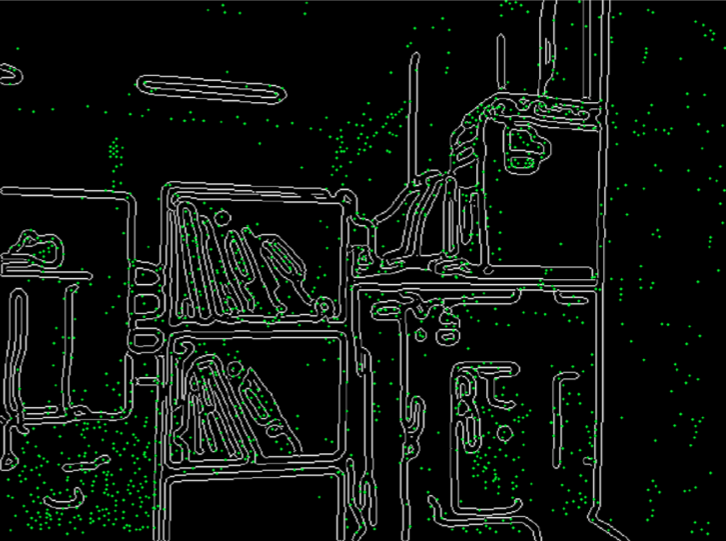
\includegraphics[resolution=150, scale=0.5]{images/lee-sift-mops-example}
  \caption{Example output for combined SIFT and MOPS features.}
  \label{fig:lee-sift-mops}
\end{figure*}

We now determine the ``type'' of the object, based on comparison of the distance of SIFT features within an outline to the distance to MOPS features on the outline. Define $D_M$ to be the distance to a MOPS feature, and $D_S$ to be the distance to a SIFT feature within the outline. Let $T_1$ and $T_2$ be two threshold values. We have the following equations
\begin{equation}
  \label{eq:dist1}
  | D_M - D_S | \leq T_1
\end{equation}
\begin{equation}
  \label{eq:dist2}
  T_1 < | D_M - D_S | \leq T_2
\end{equation}
\begin{equation}
  \label{eq:dist3}
  T_2 < | D_M - D_S |
\end{equation}

$T_1$ should be set such that there is a high probabilitiy that the SIFT and MOPS features are on the same object, and $T_2$ such that there is a high probability that the features are on different objects. We thus have the following cases:
\begin{itemize}
\item Equation~\ref{eq:dist1} is the case of an object with a closed interior.
\item Equation~\ref{eq:dist2} is again the case where an object has a closed interior, but possibly with a convex shape.
\item Equation~\ref{eq:dist3} is the case of an object with an open interior.
\end{itemize}
In the third case, we repeat the above process feature points on an object behind the open space.

This comparison allows us to determine what sort of obstacle an object is and to locate where in the world the objects exist, relative to the quadrotor.

\subsection{Replacing MOPS with Contours}
After finding object outlines using MOPS features to not give an insufficient amount of information, we sought an 
alternative approach.  As~\cite{suzuki1985} has been widely tested and locates contours within an image it appeared to be 
sufficient to meet our needs. We used the Canny Edge Detector~\cite{canny1986} to convert to binary images as the input to
this method.  After locating the contours in an image we marked the key points found using the SIFT algorithm as 
belonging to an object outline and proceeded as normal through the rest of the approach of~\cite{lee2011} as normal.

\subsection{Integrating PTAM}
Integrating PTAM with the quadrotor is remarkably simple. We made use of two different methods to accomplish this, in order to have different features available. Both methods rely upon the Robot Operating System (ROS) *** CITE ROS *** for support and the ardrone\_autonomy *** CITE ardrone\_autonomy *** driver for communication with the quadrotor.

Our first approach is to directly test PTAM on data from the quadrotor. For this, we made use of the ethzasl\_ptam package *** CITE ethzasl\_ptam ***, which integrates PTAM with ROS. It was then only a matter of converting the camera stream from the ardrone\_autonomy driver to the requisite format for use with PTAM and calibrating the camera appropriately.

Secondly, we made use of the tum\_ardrone *** CITE tum\_ardrone *** package for ROS, which integrates a version of PTAM with an extended Kalman filter for data fusion and state estimation and a system for generating steering commands for the quadrotor. tum\_ardrone builds upon PTAM to provide an environment specifically designed for use with the ARDrone and ARDrone 2, and in addition to obstacle detection, provides a system for navigation and auto-pilot.

\section{Experiments}
Our data sets consist of samples obtained by recording output from the quadrotor's forward-facing camera. These are $640 \times 360$ pixel colour images saved in JPEG format recorded at a rate of one per each $0.01$ second. Our initial data sets consisted of
\begin{itemize}
\item A set of 212 frames in which the drone is sitting still on a table.
\item A set of 321 frames in which the drone takes off, flies down a Siebel Center hall, and lands.
\item A set of 301 frames in which the drone takes off, flies through the Siebel Center atrium, and lands.
\end{itemize}
These were supplemented with the following additional data sets from the quadrotor, this time recorded at a rate of one per each $0.1$ second.
\begin{itemize}
\item A set of 130 frames in which the drone flies through the Siebel Center atrium with additional movement, and people present.
\item A set of 275 frames in which the drone flies closely along the pillars and display cases of in the Siebel Center atrium.
\item A set of 49 frames in which the drone flies towards a corner in the Siebel Center atrium.
\end{itemize}

\subsection{Lee et al.}


\subsection{PTAM}


\begin{figure*}[h]
  \centering
  \begin{tabular}{cc}
    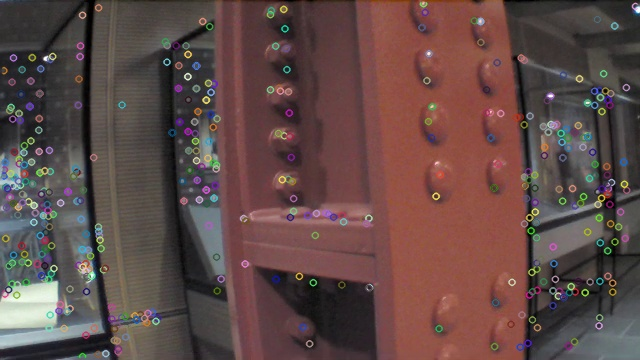
\includegraphics[resolution=150, scale=0.75]{images/sift-kp1} &
    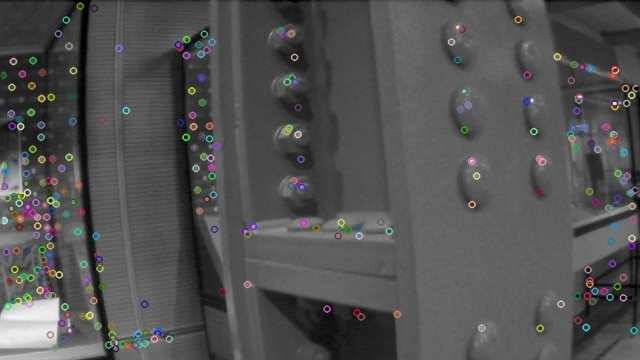
\includegraphics[resolution=150, scale=0.75]{images/sift-kp2} \\
    \multicolumn{2}{c}{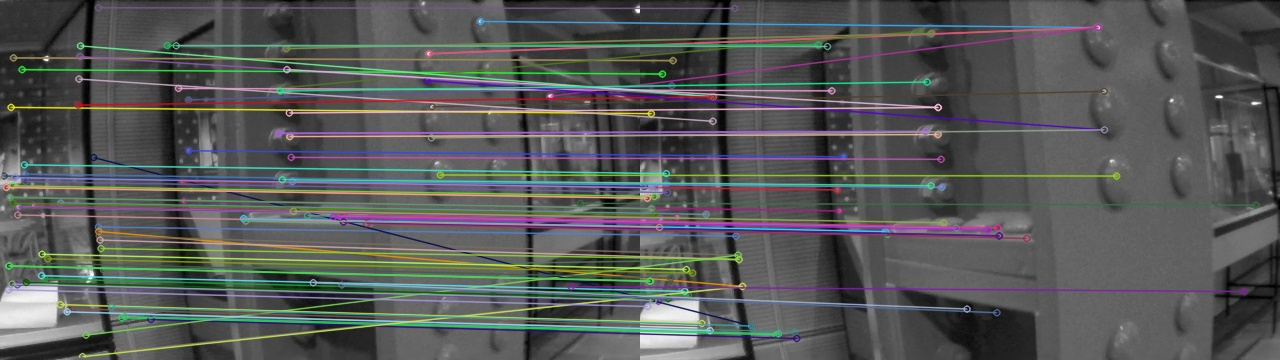
\includegraphics[resolution=150, scale=0.75]{images/sift-matches}}
  \end{tabular}
  \caption{SIFT keypoints and matches.}
  \label{fig:sift-ex}
\end{figure*}

\begin{figure*}[h]
  \centering
  \begin{tabular}{cc}
    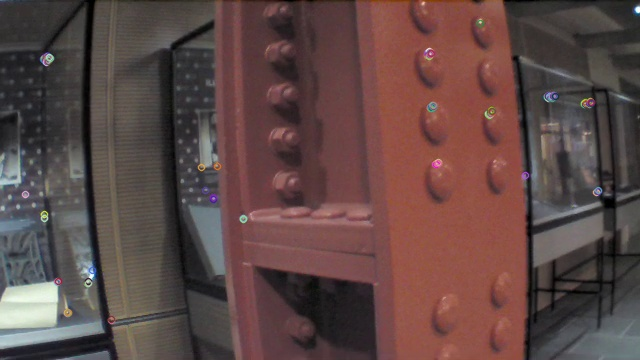
\includegraphics[resolution=150, scale=0.75]{images/mops-kp1} &
    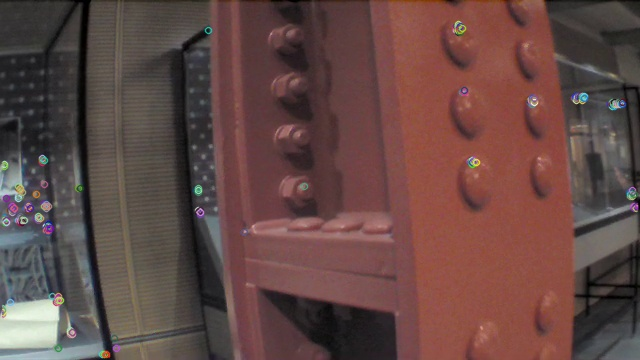
\includegraphics[resolution=150, scale=0.75]{images/mops-kp2} \\
    \multicolumn{2}{c}{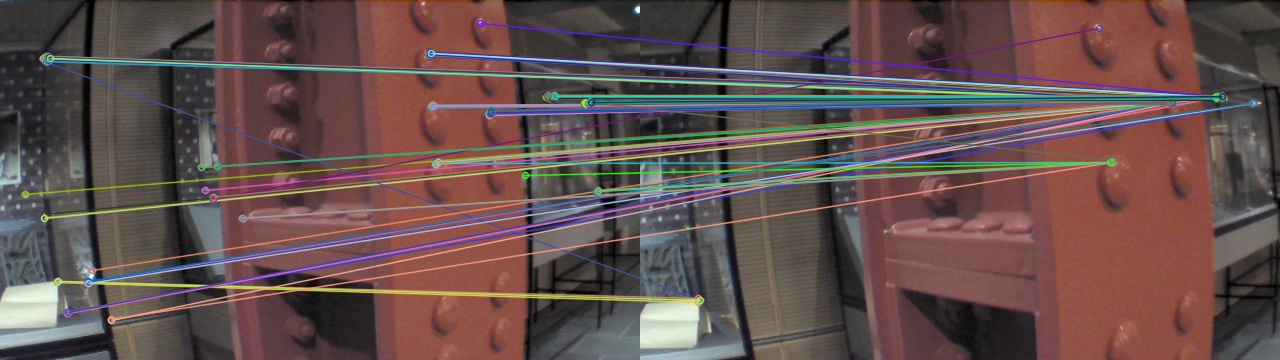
\includegraphics[resolution=150, scale=0.75]{images/mops-matches}}
  \end{tabular}
  \caption{MOPS keypoints and matches.}
  \label{fig:mops-ex}
\end{figure*}

\begin{figure*}[h]
  \centering
  \begin{tabular}{cc}
    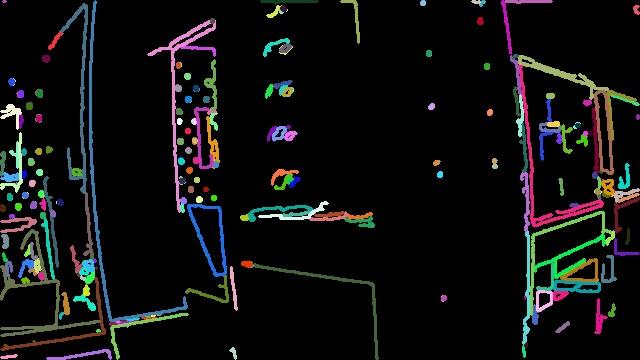
\includegraphics[resolution=150, scale=0.75]{images/contour-lines1} &
    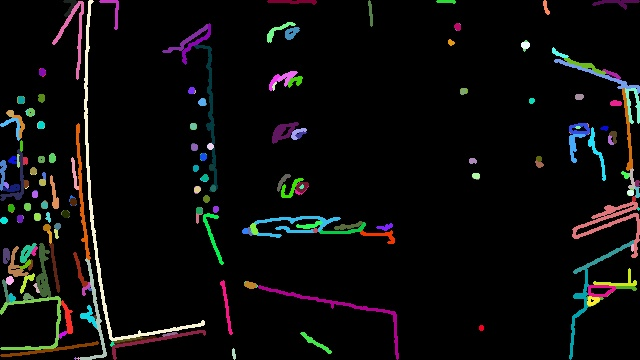
\includegraphics[resolution=150, scale=0.75]{images/contour-lines2} \\
    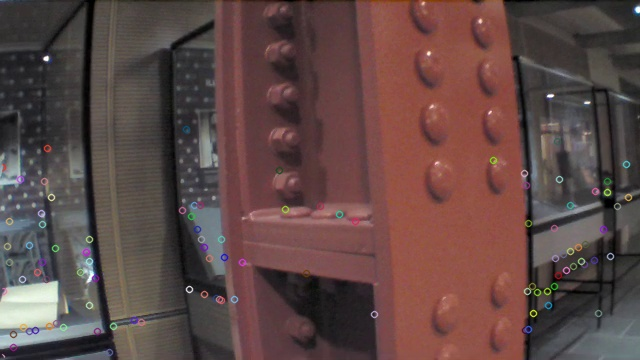
\includegraphics[resolution=150, scale=0.75]{images/contour-kp1} &
    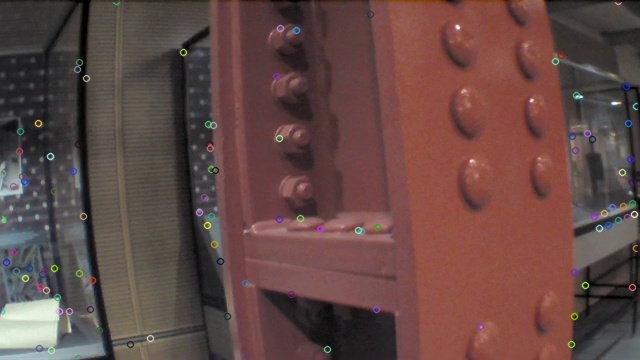
\includegraphics[resolution=150, scale=0.75]{images/contour-kp2} \\
    \multicolumn{2}{c}{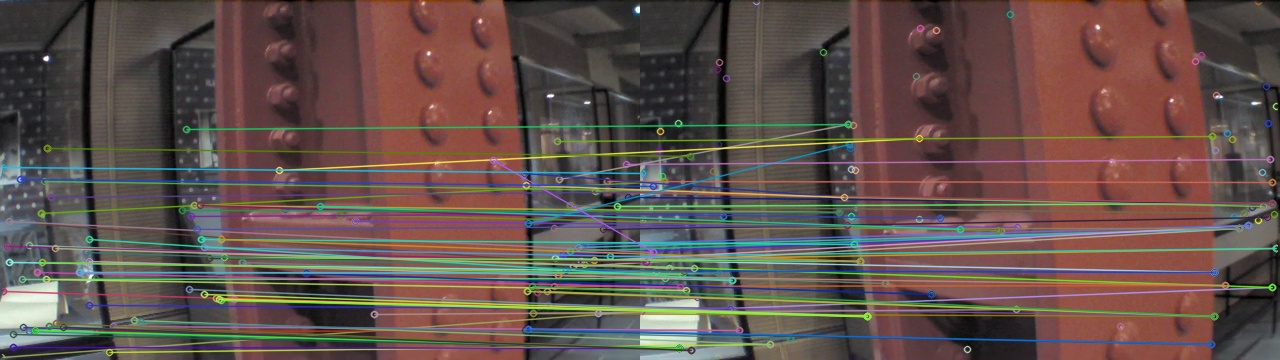
\includegraphics[resolution=150, scale=0.75]{images/contour-matches}}
  \end{tabular}
  \caption{Contour lines, keypoints, and matches.}
  \label{fig:contour-ex}
\end{figure*}

\begin{figure*}[h]
  \centering
  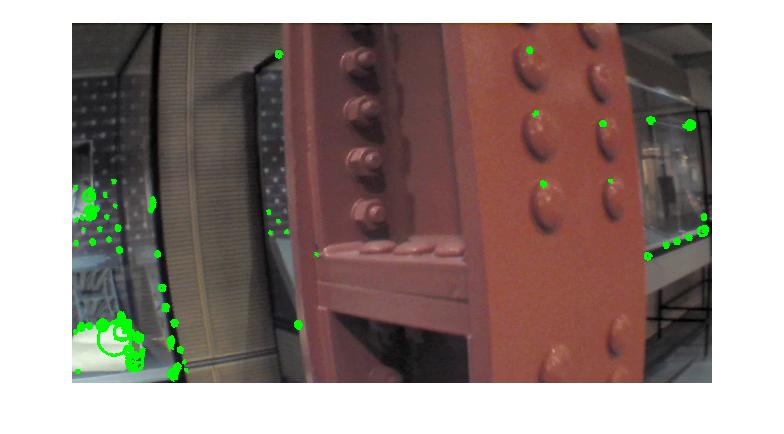
\includegraphics[resolution=150, scale=0.75]{images/vlfeat-kp2}
  \caption{VLFeat multi-scale Harris corner detector keypoints.}
  \label{fig:vlfeat-ex}
\end{figure*}

\section{Analysis}


\section{Individual Contributions}
Individual contributions break down roughly as follows. Nikoli was responsible for:
\begin{itemize}
\item Implementing SIFT feature detection, extraction, and image matching
\item Implementing 3-D reconstruction and triangulation
\item Implementing the multi-threaded image pipeline
\item Setting up and integrating ethzasl\_ptam with the quadrotor
\item Setting up tum\_ardrone
\item Experimental evaluations
\item Presentation and paper writing
\end{itemize}

Bryan was responsible for:
\begin{itemize}
\item Implementing MOPS feature detection, extraction, and image matching
\item Experimenting with a contour-based technique to replace MOPS
\item Assistance with 3-D reconstruction
\item Assistance with setting up ethzasl\_ptam
\item Experimental evaluations
\item Presentation and paper writing
\end{itemize}

Because MOPS was implemented from scratch, we feel that the work was split quite evenly.

\bibliographystyle{acmsiggraph}
\bibliography{bib_all}
\end{document}


